%\documentclass[notes,11pt,aspectratio=169]{beamer}
\documentclass[11pt,aspectratio=169]{beamer}
\usetheme{auriga} %Themes http://www.hartwork.org/beamer-theme-matrix/
\usecolortheme{auriga}


\definecolor{red}{RGB}{255, 0, 0}
\definecolor{blue}{RGB}{0, 118, 186}
\definecolor{green}{RGB}{0,255,0}
\definecolor{gray}{RGB}{146, 146, 146} 
\definecolor{colorA}{RGB}{96, 34, 59}
\definecolor{colorB}{RGB}{140, 151, 154}

\definecolor{secinhead}{RGB}{249,196,95}
\definecolor{titlebg}{RGB}{51,51,51}
%\setbeamercolor{structure}{fg=colorA,bg=colorB}
\setbeamercolor{secsubsec}{fg=secinhead,bg=black}
%\setbeamercolor{frametitle}{fg=secinhead,bg=red}
\setbeamercolor{block title}{fg=red}




%=================================================
% packages and new commands
%=================================================
\usepackage[ruled, linesnumbered, vlined]{algorithm2e}
\usepackage{multirow, algorithmic, amsmath}
\usepackage[french]{babel} % babel system, adjust the language of the content
\usepackage{animate}
\usepackage{fontawesome5}

\usepackage{pgfpages}
\usepackage{fancyvrb}
\usepackage{tikz}
\usepackage{pgfplots}
\usepackage{tikz}
\usetikzlibrary{trees}
\usetikzlibrary{arrows, decorations.markings}

\usetikzlibrary{shadows}

\usepackage{transparent,graphicx,xcolor}



\setbeamertemplate{note page}[plain]

%\setbeameroption{show notes}
%\setbeameroption{show notes on second screen=right}


%% Beamer pass-through options
\DeclareOptionBeamer{compress}{\beamer@compresstrue}
\DeclareOptionBeamer{deutsch}{\@uzhdeutschtrue}
\DeclareOptionBeamer{german}{\@uzhdeutschtrue}
\ProcessOptionsBeamer

%% Theme options
\DeclareOption{deutsch}{\@uzhdeutschtrue}
\DeclareOption{german}{\@uzhdeutschtrue}
\DeclareOption{informal}{\@uzhinformaltrue}
\DeclareOption{formal}{\@uzhinformalfalse}
\ProcessOptions


% fonts

\newcommand\importantstuff[3]{
	\node[black!30!white] at (#1+0.1,#2-0.1) {
		\scalebox{2}{\Huge\texttt{#3}} 
	};
	\node at (#1,#2) {
		\scalebox{2}{\Huge\texttt{#3}} 
	};
}

\RequirePackage{eulervm}% math font that blends better with Bookman
\setbeamerfont{title}{size={\fontsize{20}{24pt}\selectfont},parent=structure,series=\bfseries}
\setbeamerfont{subtitle}{size={\fontsize{9}{11pt}\selectfont},series=\mdseries}
\setbeamerfont{author}{size={\fontsize{9}{11pt}\selectfont},series=\mdseries}
\setbeamerfont{footline}{size={\fontsize{5}{7pt}\selectfont}}% originally also: shape=\itshape
\setbeamercolor{footline}{fg=black}
\setbeamerfont{frametitle}{parent=structure,size={\fontsize{12}{14pt}\selectfont},series=\bfseries}
\setbeamerfont{framesubtitle}{parent=frametitle,size=\footnotesize}
\setbeamerfont{uzhunit}{size={\fontsize{7}{9pt}\selectfont},series=\bfseries,family=\sffamily}




\tikzstyle{vecArrow} = [thick, decoration={markings,mark=at position
	1 with {\arrow[semithick]{open triangle 60}}},
double distance=1.4pt, shorten >= 5.5pt,
preaction = {decorate},
postaction = {draw,line width=1.4pt, white,shorten >= 4.5pt}]
\tikzstyle{innerWhite} = [semithick, white,line width=1.4pt, shorten >= 4.5pt]


\tikzstyle{every picture}+=[remember picture]

% By default all math in TikZ nodes are set in inline mode. Change this to
% displaystyle so that we don't get small fractions.
\everymath{\displaystyle}

\usetikzlibrary{calc,fadings}
\tikzfading[name=fade l,left color=transparent!100,right color=transparent!0]
\tikzfading[name=fade r,right color=transparent!100,left color=transparent!0]
\tikzfading[name=fade d,bottom color=transparent!100,top color=transparent!0]
\tikzfading[name=fade u,top color=transparent!100,bottom color=transparent!0]

% this "frames" a rectangle node
\newcommand\framenode[2][10pt]{
	\fill[white,path fading=fade u] (#2.south west) rectangle ($(#2.south east)+(0, #1)$);
	\fill[white,path fading=fade d] (#2.north west) rectangle ($(#2.north east)+(0,-#1)$);
	\fill[white,path fading=fade l] (#2.south east) rectangle ($(#2.north east)+(-#1,0)$);
	\fill[white,path fading=fade r] (#2.south west) rectangle ($(#2.north west)+( #1,0)$);
}

\makeatletter
\let\insertsupervisor\relax
\newcommand\supervisortitle{Sous la direction de}
\mode<all>
{
	\newcommand\supervisor[1]{\def\insertsupervisor{#1}}
	\titlegraphic{}
}
\defbeamertemplate*{title page}{supdefault}[1][]
{
	\vbox{}
	\vfill
	\begingroup
	\centering
	\begin{beamercolorbox}[sep=8pt,center,#1]{title}
		\usebeamerfont{title}\inserttitle\par%
		\ifx\insertsubtitle\@empty\relax%
		\else%
		\vskip0.25em%
		{\usebeamerfont{subtitle}\usebeamercolor[fg]{subtitle}\insertsubtitle\par}%
		\fi%     
	\end{beamercolorbox}%
	\vskip1em\par
	\begin{beamercolorbox}[sep=8pt,center,#1]{author}
		\usebeamerfont{author}\insertauthor
	\end{beamercolorbox}
	\ifx\insertsupervisor\relax\relax\else
	\begin{beamercolorbox}[sep=8pt,center,#1]{}
		\usebeamerfont{author}\supervisortitle:~\insertsupervisor
	\end{beamercolorbox}\fi
	\begin{beamercolorbox}[sep=8pt,center,#1]{institute}
		\usebeamerfont{institute}\insertinstitute
	\end{beamercolorbox}
	\begin{beamercolorbox}[sep=8pt,center,#1]{date}
		\usebeamerfont{date}\insertdate
	\end{beamercolorbox}\vskip0.5em
	
	{\usebeamercolor[fg]{titlegraphic}\inserttitlegraphic\par}
	\endgroup
	\vfill
}

\title[ \hspace{0.8cm} \insertframenumber/\inserttotalframenumber]{{\sc Interview for PhD thesis with Prof. Farida Fassi}}


 
\author{{ Ismail EZZAKI}}


\newcommand*{\rom}[1]{\expandafter\@slowromancap\romannumeral #1@}




%=================================================
% start presentation
%=================================================
\begin{document}

\setbeamertemplate{titlepage}[supdefault]

{
	% rather than use the frame options [noframenumbering,plain], we make the
	% color match, so that the indicated page numbers match PDF page numbers
	%\setbeamercolor{page number in head/foot}{fg=background canvas.bg}
	\begin{frame}
		\begin{center}	%\includegraphics[width=0.9\linewidth,height=0.2\textheight]{figures/header.png}\\
		\end{center}

		\titlepage
	\end{frame}
}
%\begin{frame}
%
%	\frametitle{Outline 
%	}
%	\tableofcontents
%\end{frame}

%========================
% your slides:
%========================




\section{About me}

\begin{frame}{\underline{\secname}}

	\begin{center}
		\textbf{About me}
	\end{center}

	%\animategraphics[autoplay,loop,height=5cm]{1}{my_ongfile_}{0}{n-1}

	\begin{itemize}
		\item Full name : Ismail EZZAKI
		\item Age : 24 years old
		\item Country : Morocco
		\item I’ve always been interested in discovering how things work $\rightarrow$ physics
		\item Childhood dream (age =< 12 yrs): Win a Nobel prize in physics
		\item Realistic dream (age > 12 yrs): Be an academic researcher in physics
	\end{itemize}


\end{frame}






\begin{frame}{\underline{\secname}}

	\begin{center}
		\textbf{Academic background}
	\end{center}
	\begin{columns}
		\begin{column}{0.5\linewidth}

			\begin{itemize} 			  \setlength\itemsep{0em}

				\item 2014: High School in Experimental sciences
				\item 2018: B.Sc. in Fundamental Physics

				\item 2020: M.Sc. in High energy physics and computational physics
			\end{itemize}

		\end{column}

		\pause
		\begin{column}{0.5\linewidth}

			\begin{itemize}			  \setlength\itemsep{0em}

				\item 2014: Programming
				\item 2018: Machine / Deep learning
			\end{itemize}
		\end{column}
	\end{columns}
	\pause
	\begin{center}
		\textbf{Skills}
	\end{center}
	\begin{itemize}			  \setlength\itemsep{0em}
		\item
		      theoretical knowledge in particle physics

		\item
		      Programming ( Python \& C++ \& Javascript...)

		       \item  DevOps : Docker , Git , Testing and Debugging , CMake , CI/CD
		      
		\item Soft Skills: Problem solving and logical thinking %, working with large team project 


		      % \item
		      % working with large team project - 
		      % - Software testing and debugging


		      % 
		      % ////////////

		      % //////////////////
		      % 
		      % 
		      % 
% TODO “Each day, I spend the first 15 to 30 minutes checking which tasks are left in my sprint, communicating with my supervisor and fellow software engineers to see what tasks are ready for me to start. Then, I prioritize each task based on when it needs to be completed. Finally, I determine how long each task will take and ensure that each task can fit within my hours worked that day.”
		      % 
		      % Did your research projects involve programming?



	\end{itemize}

	\begin{itemize}			  
	\item My current research interest is :\textbf{ data analysis in particle physics \& computational physics }
	
\end{itemize}
\end{frame}

%
%\begin{frame}{\underline{\secname}}
%	
%	\begin{center}
%		\textbf{Spare time activities}
%	\end{center}
%	
%	\begin{center}
%		\textbf{}
%	\end{center}
%	\begin{columns}
%		\begin{column}{0.5\linewidth}
%			
%			\begin{figure}
%				\centering
%				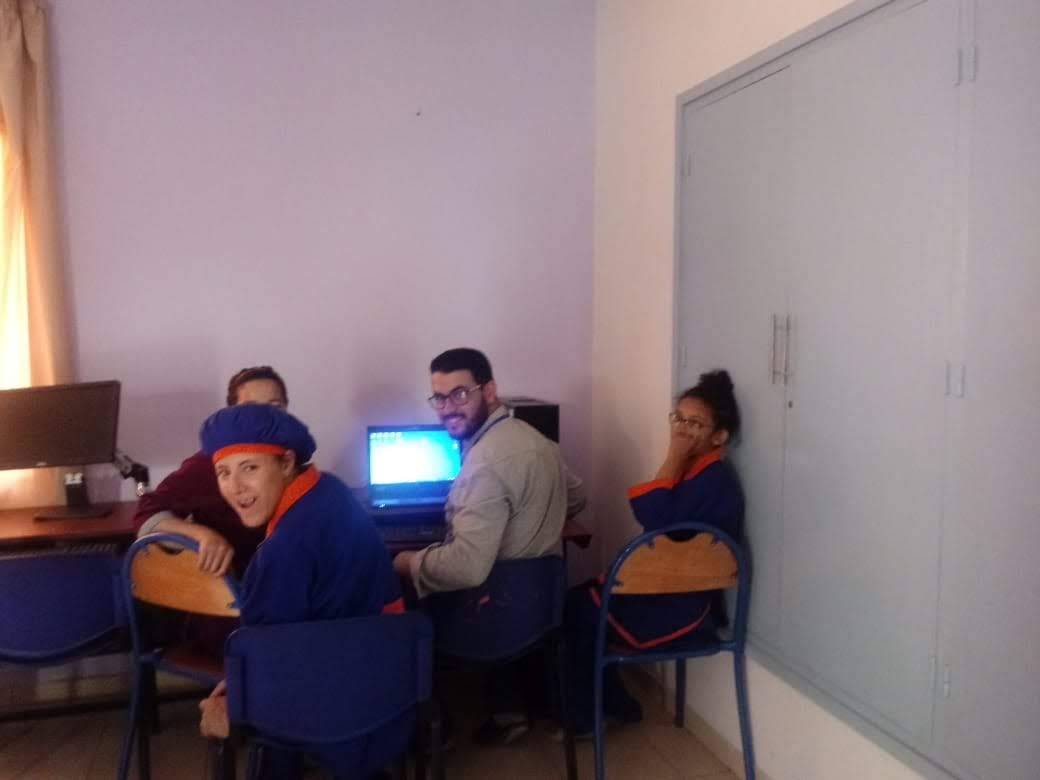
\includegraphics[width=1.2\linewidth,height=130pt]{figures/IMG-20190510-WA0014.jpg}
%			\end{figure}
%		\end{column}
%		
%		\begin{column}{0.5\linewidth}
%			
%			\begin{figure}
%				\centering
%				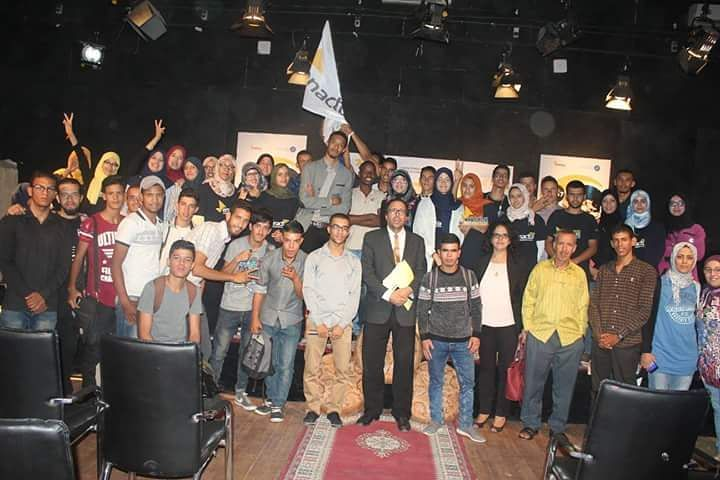
\includegraphics[width=1.2\linewidth,height=130pt]{figures/enactus}
%			\end{figure}
%		\end{column}
%	\end{columns}
%	
%	|
%\end{frame}

%
\section{Research Interests \& Experience}


\begin{frame}{\underline{\secname}}


\begin{center}
\textbf{GANs to simulate Drell-Yan  events in  ATLAS experiment}
\end{center}

\begin{itemize}			  \setlength\itemsep{0em}

\item GAN: A two- Deep NN game where one genrate events (generator) and one (discriminator) classifies events as real (from real simulation ) or fake (from the generator)

\item the game ends when the generator success to fool the discriminator = the generator can produce events similar to a real simulation

\item GANs can learn complex P(x)

\item GANs provide a viable strategy for speeding up numerically intensive simulation

\end{itemize}
\begin{figure}[H]
\begin{center}
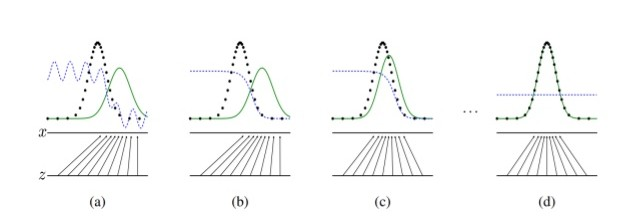
\includegraphics[width=0.6\textwidth]{figures/gauss.jpg}
\end{center}
\end{figure}

\end{frame}



\begin{frame}{\underline{\secname}}


\begin{center}
\textbf{Preparing the dataset}
\end{center}
\begin{itemize}			  \setlength\itemsep{0em}

\item
Considering a sample of $Z \to \mu \mu$ events in proton-proton collisions,
\item
generated using the {\tt PYTHIA8} event generator at a center-of-mass energy of 13~TeV.
\item
Detector resolution and efficiency are taken into account using the parametric description of the ATLAS detector provided by the {\tt DELPHES} detector simulation library.
\item
Events are generated with an average of 20 simultaneous collisions (pileup)
\item \textbf{Problems} : Choosing the number of features - choosing coordinate system - finding the best GAN structure

\end{itemize}

\end{frame}



\begin{frame}{\underline{\secname}}

%A rotation of the two four-momenta is applied, so that $p_y^{\mu 1}=0$, after the rotation. Once this is done, $p_y^{\mu 1}$ is discarded from the dataset.

\begin{center}
\textbf{Preparing the dataset}
\end{center}

\begin{figure}[H]
\begin{center}
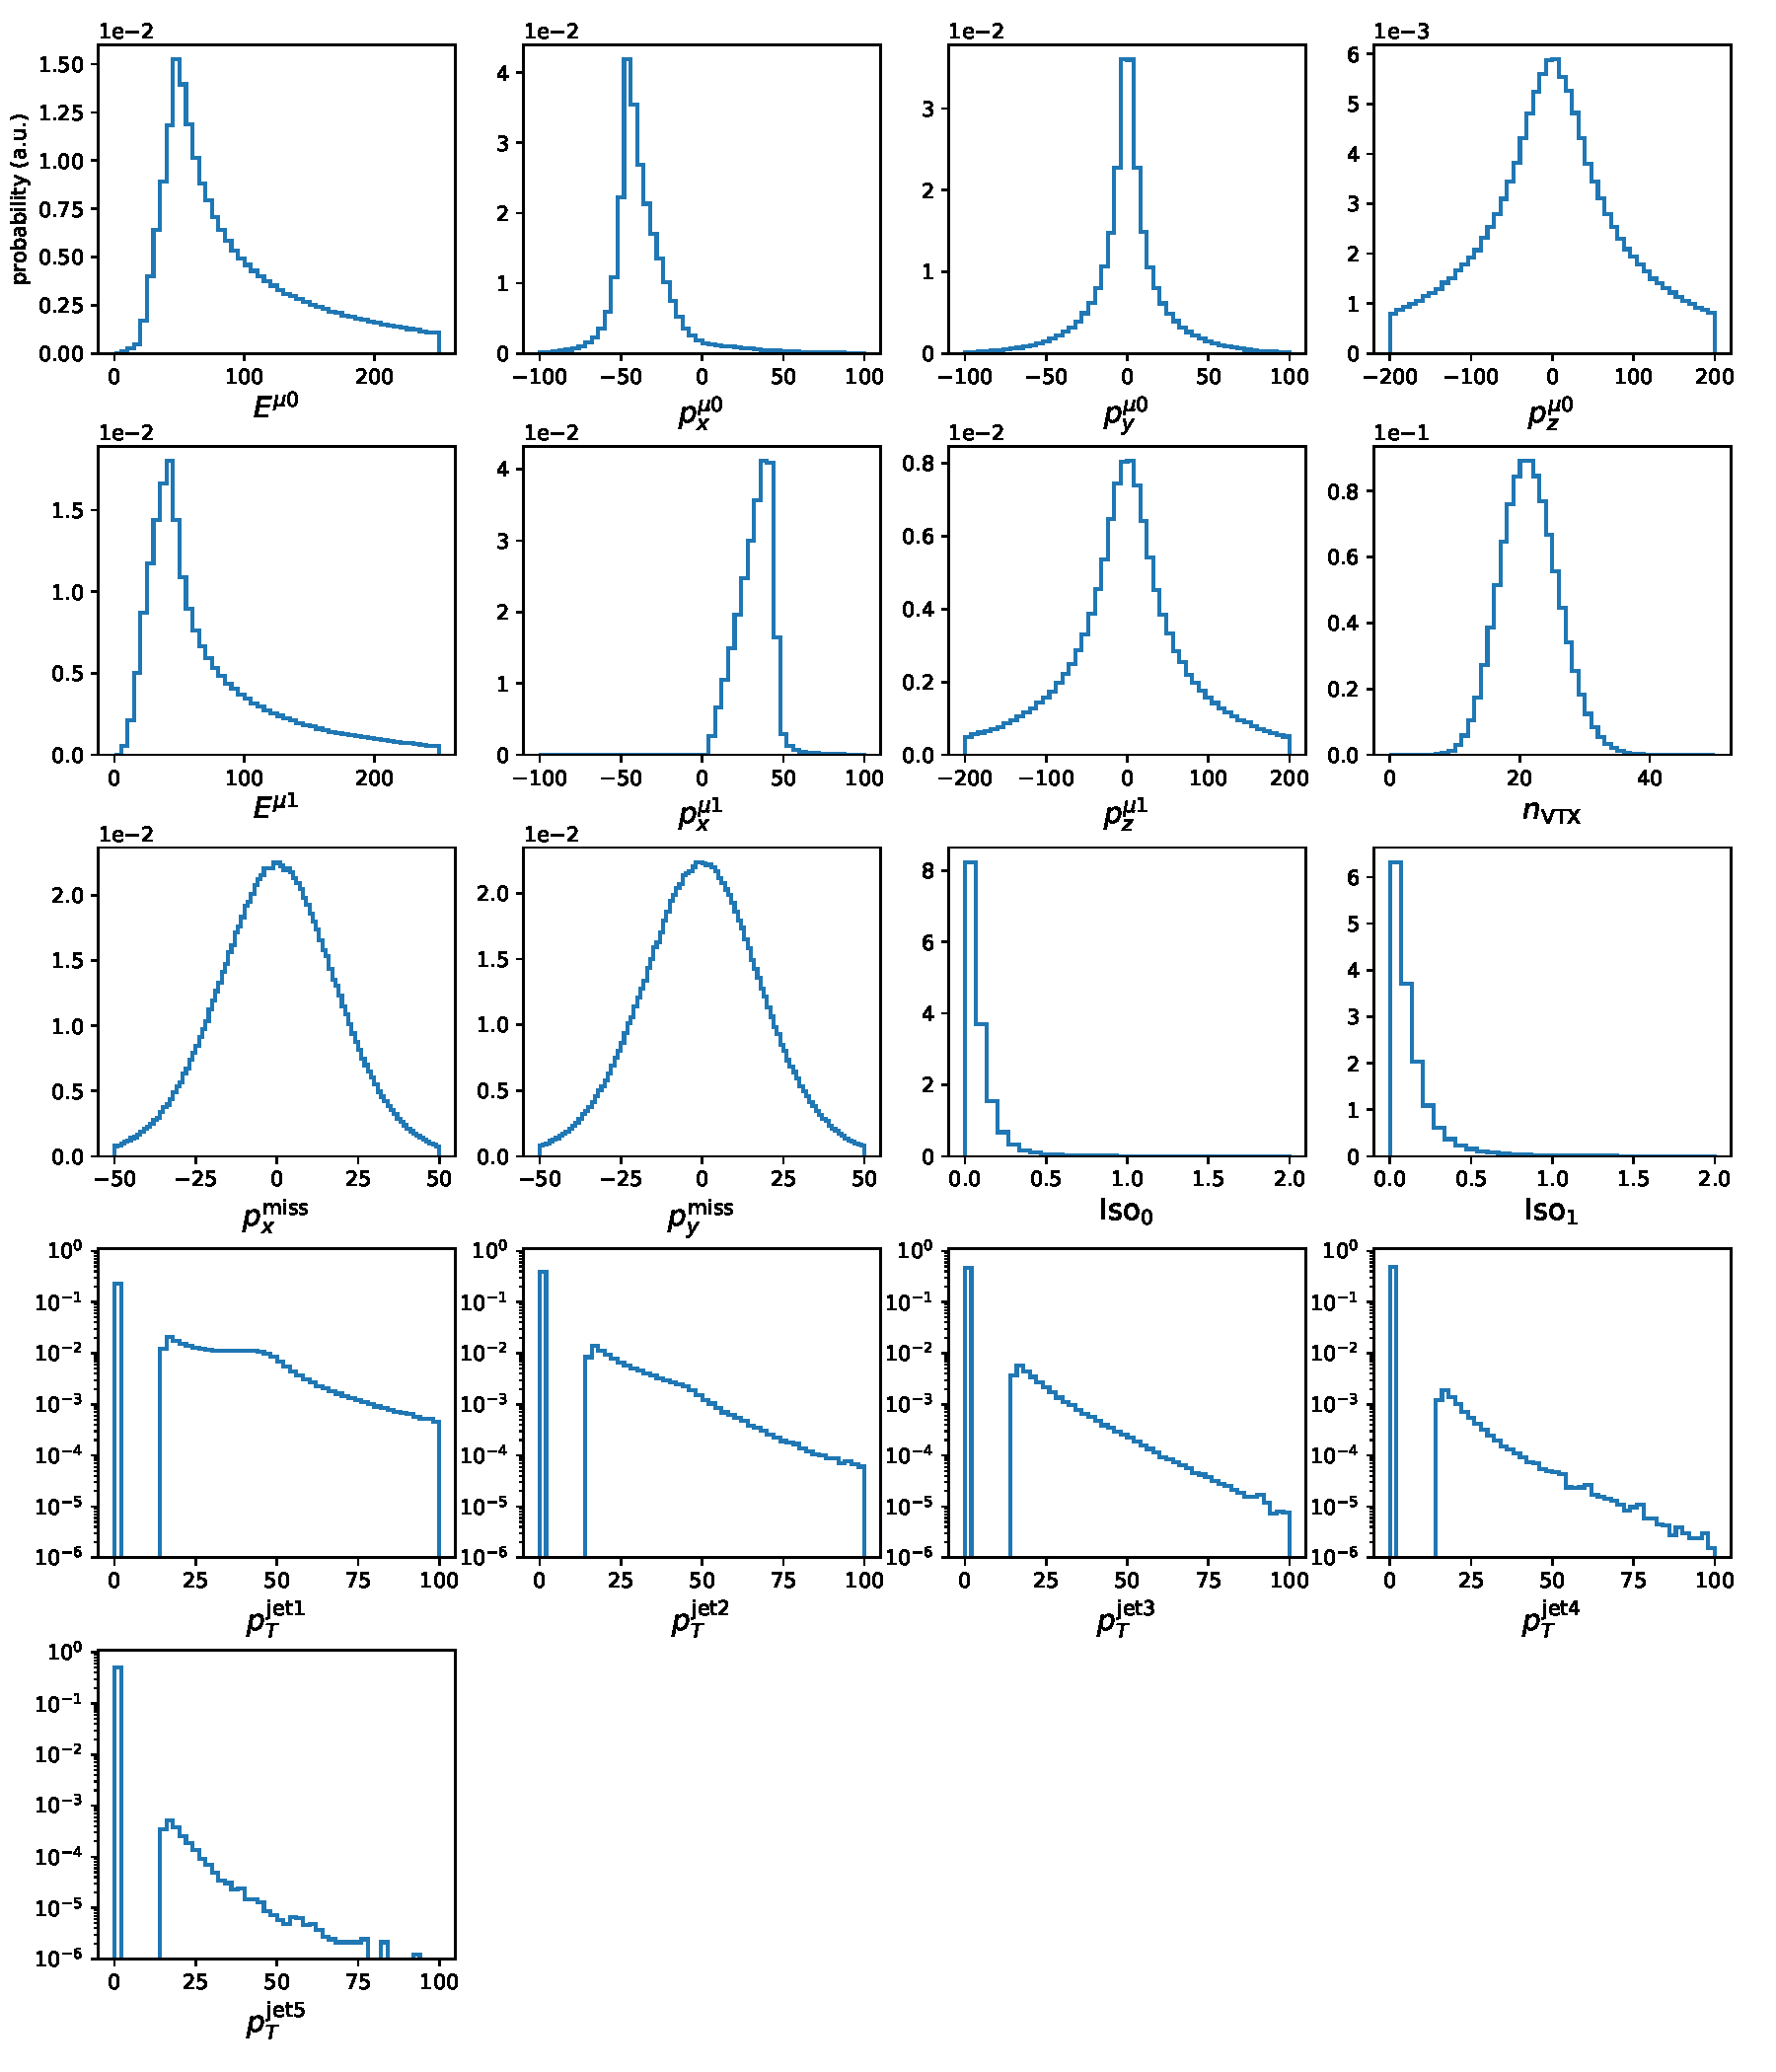
\includegraphics[width=0.4\textwidth]{slides/plotmatrix_realonly_train}
\end{center}
\end{figure}

\end{frame}


\begin{frame}{\underline{\secname}}

%A rotation of the two four-momenta is applied, so that $p_y^{\mu 1}=0$, after the rotation. Once this is done, $p_y^{\mu 1}$ is discarded from the dataset.

\begin{center}
\textbf{Final dataset}
\end{center}

\begin{figure}[H]
\begin{center}
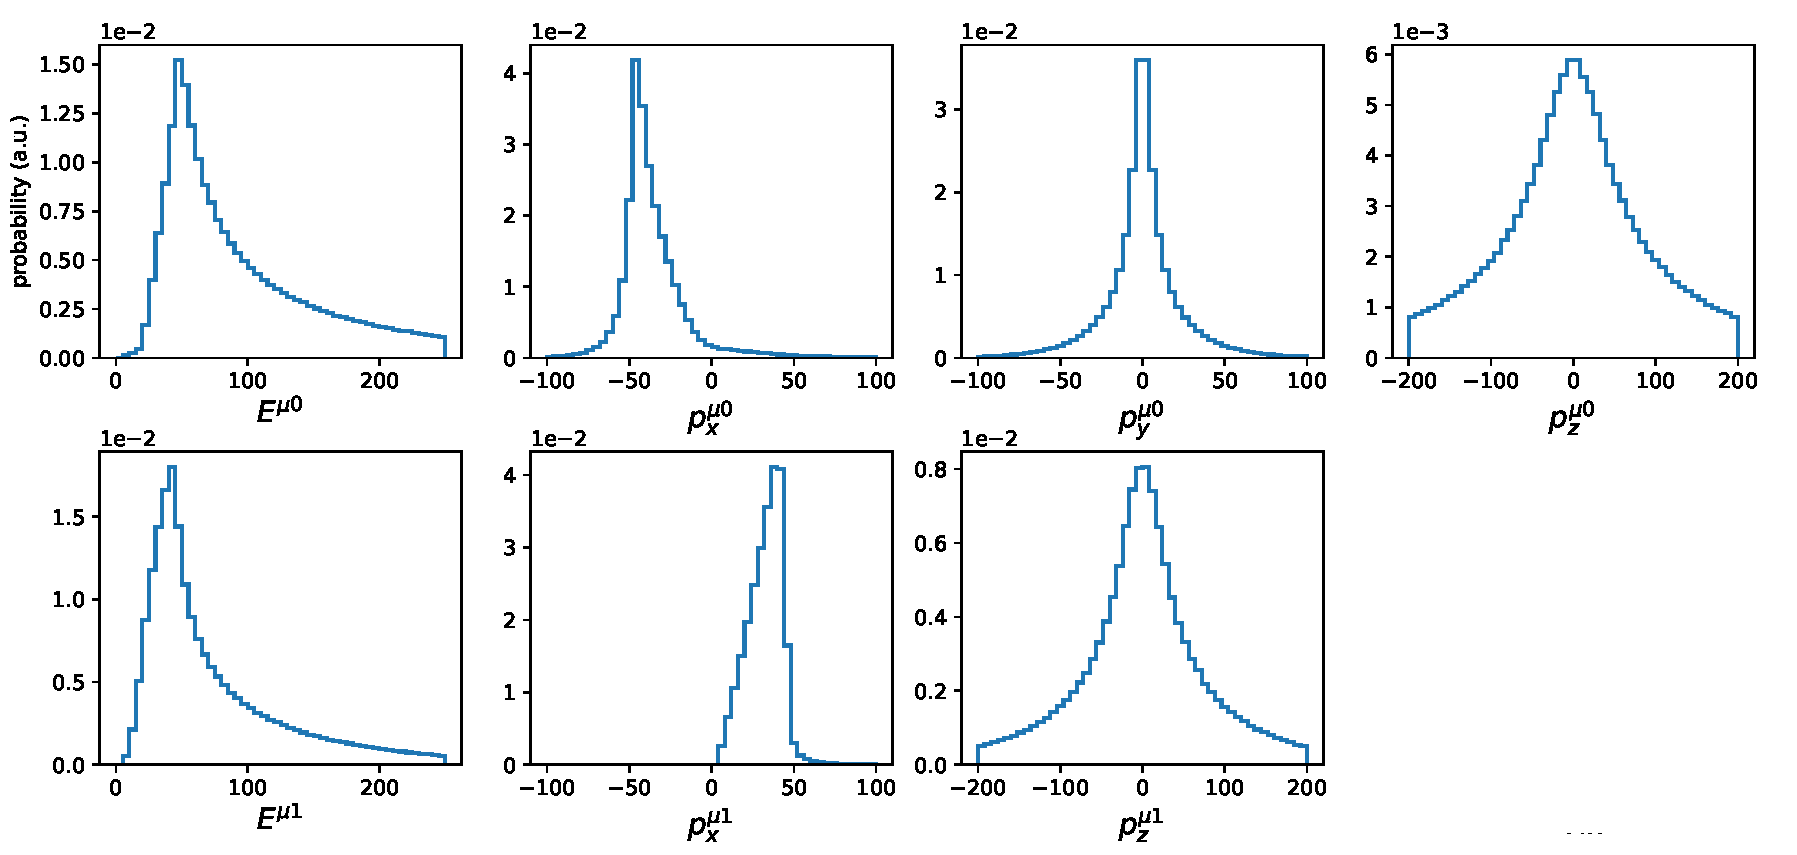
\includegraphics[width=\textwidth]{slides/pdfresizer.com-pdf-crop}
\end{center}
\end{figure}

\end{frame}

\begin{frame}{\underline{\secname}}

\begin{center}
\textbf{The GAN structure}
\end{center}
\begin{itemize}			
\item

The generator network consists of 7 fully connected layers, The input to the generator network consists of 7 ``noise'' floating-point numbers, sampled from a Gaussian distribution centered at 0 with unit variance.
% Neurons in the inner layers are activated by leaky ReLU functions, while linear activation functions are used for the output layers. 


\item

The discriminator network consists of 9 hidden dense layers % with 128, 128, 256, 256, 128, 64, 32, 16, and 8 neurons, activated by a leaky ReLU function. The last hidden layer is fully connected to a single-neuron output layer with sigmoid activation. In addition, a layer connected directly to the input layer returns the dilepton mass as part of the output.

\item

The combined network is trained adversarially for 40,000 epochs.

\item

All networks were implemented in {\tt KERAS}, using {\tt TensorFlow} as a back-end, The training was performed using Google TPU type (v2).

\end{itemize}

\end{frame}


\begin{frame}{\underline{\secname}}


\begin{center}
\textbf{The GAN structure}
\end{center}

\begin{center}
{The generator network}
\end{center}
\begin{figure}[H]
\begin{center}
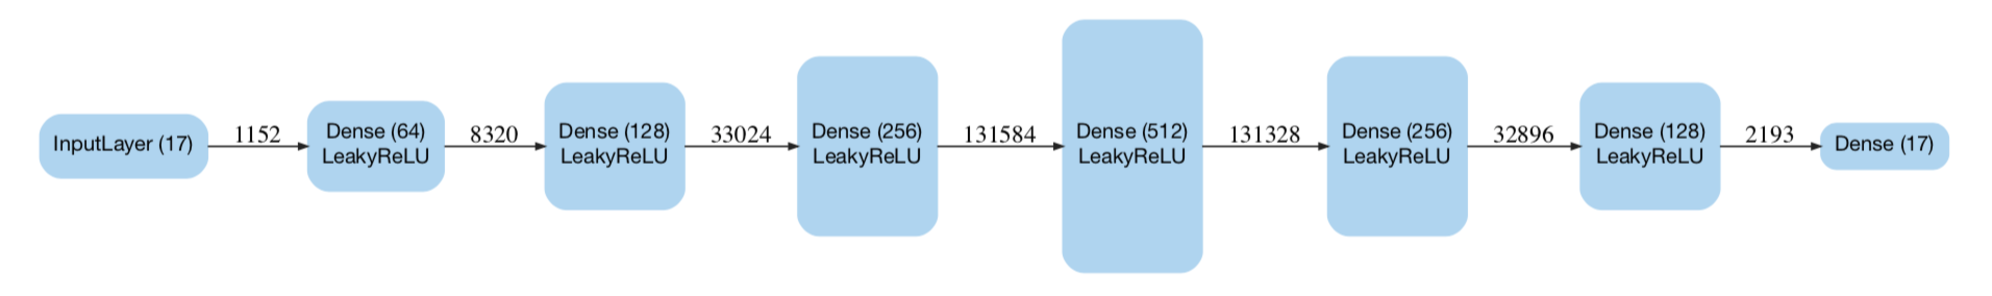
\includegraphics[width=\textwidth]{slides/generator_network}
\end{center}
\end{figure}

\begin{center}
{The discriminator network}
\end{center}

\begin{figure}[H]
\begin{center}
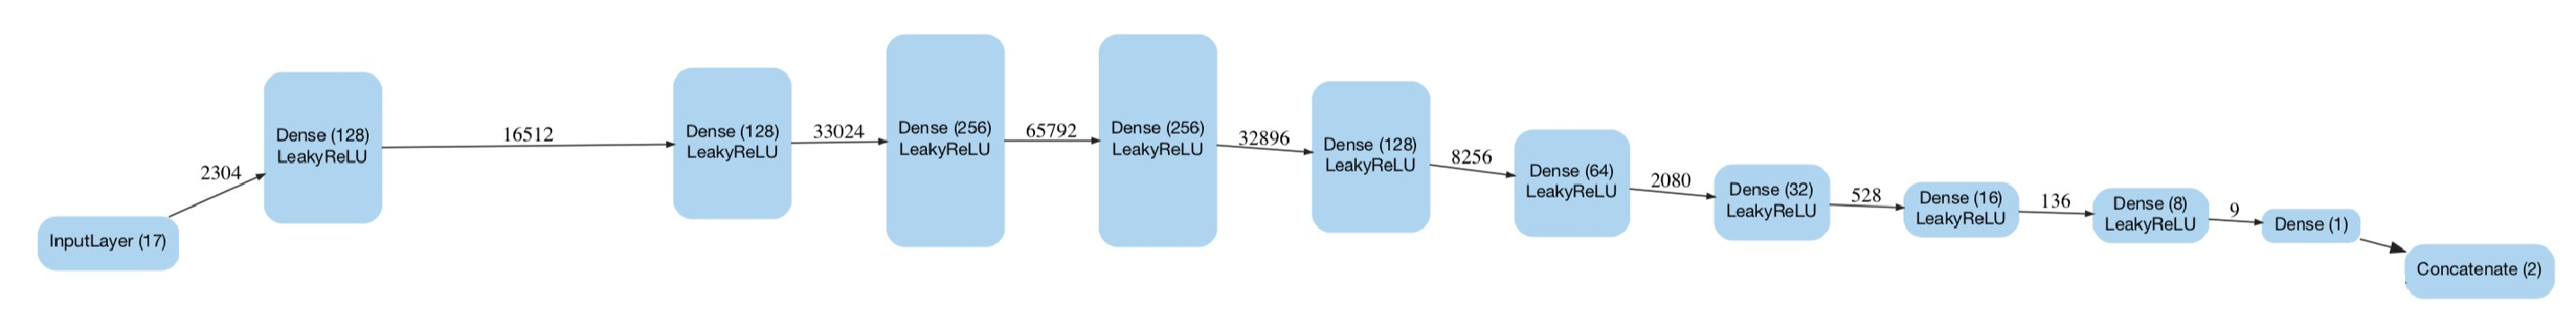
\includegraphics[width=\textwidth]{slides/discriminator_network}
\end{center}
\end{figure}

\end{frame}

\begin{frame}{\underline{\secname}}


\begin{center}
\textbf{Results}
\end{center}


\begin{figure}[H]
\begin{center}
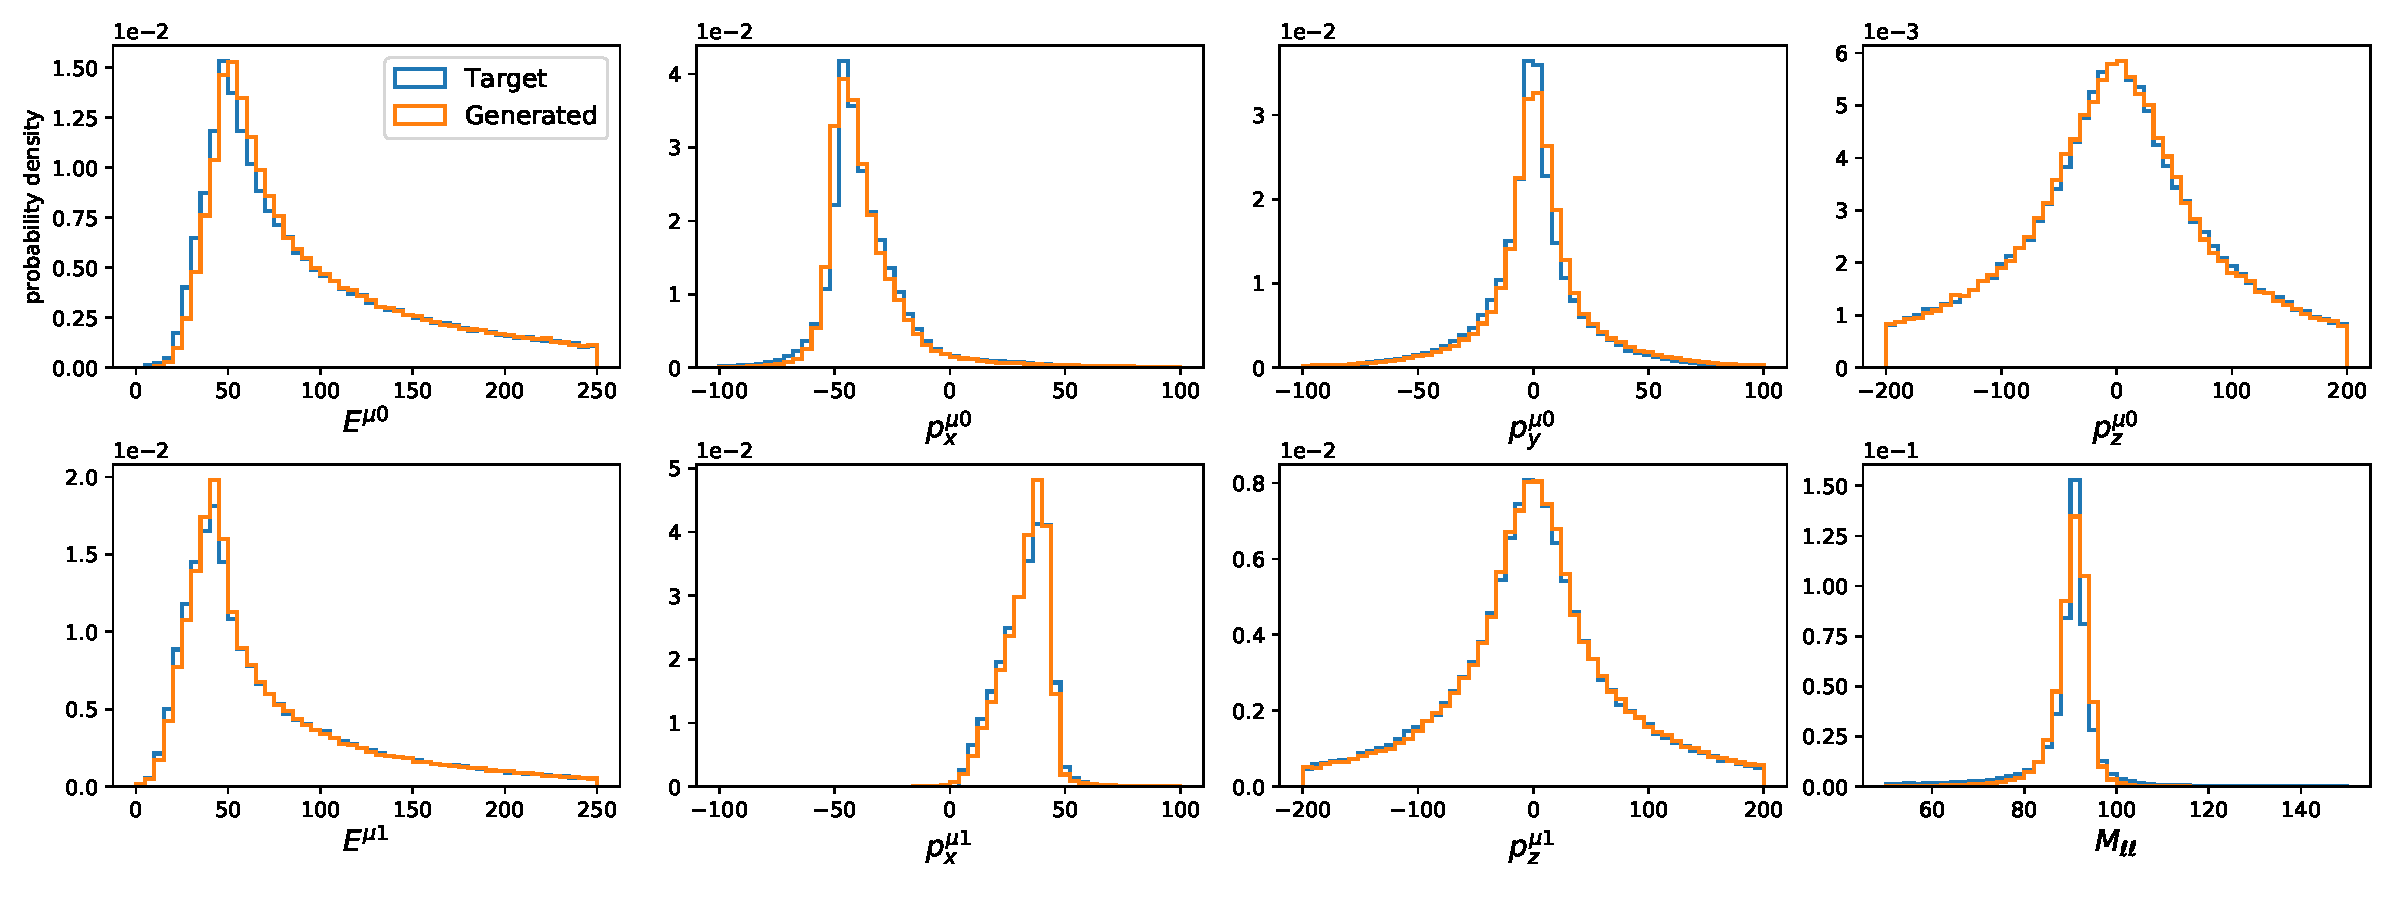
\includegraphics[width=\textwidth]{slides/trial9_epoch39700_minigantest_mllloss_final}
\end{center}
\end{figure}





\end{frame}

\begin{frame}{\underline{\secname}}


\begin{center}
\textbf{Results}
\end{center}

\begin{itemize}			  \setlength\itemsep{0em}
\item \textbf{GAN} : 5000 events/s  \t{  } \textbf{{\Large $ <<  $}}\t{  }  \textbf{DELPHES + Pythia} : 5000 events in \textit{{$\sim 3.5$ min}}
\item
Results show that GANs can learn the multi-dimensional pdf of $\cal{O}$(7) features
\item
The GAN shows problems in learning distributions with sharp features such as edges
\item
The Gan indicate a good performance but the reached precision is still insufficient to meet the precision requirements of an LHC data analysis.
\end{itemize}

\begin{center}
\textbf{Solutions}
\end{center}
\begin{itemize}			  \setlength\itemsep{0em}
\item Auxiliary GAN
\item reinforcement learning

\item  Conditional Hybrid GAN


\end{itemize}
\end{frame}
%
%\begin{frame}{\underline{\secname} : Other computational Projects}
%	\begin{columns}
%		\begin{column}{0.5\linewidth}
%
%	\begin{itemize}			  \setlength\itemsep{0em}
%		\item \textbf{Higgs ML }: signal / background separation using RNN and Xgboost instead of BDT
%		\item \textbf{Epidemic simulation} : a simulation using Pygame to show people why they need to stay at home and help Flattening the curve
%		\item \textbf{Also} : websites using Javascript \& ml modules using Python \& open source projects
%		
% 
%\end{itemize}
%		\end{column}
%
%		\begin{column}{0.5\linewidth}
%
%			
%			% \animategraphics[loop,width=\textwidth]{10}{slides/New Folder/something-}{0}{16}
%
%			\begin{figure}[H]
%				\begin{center}
%					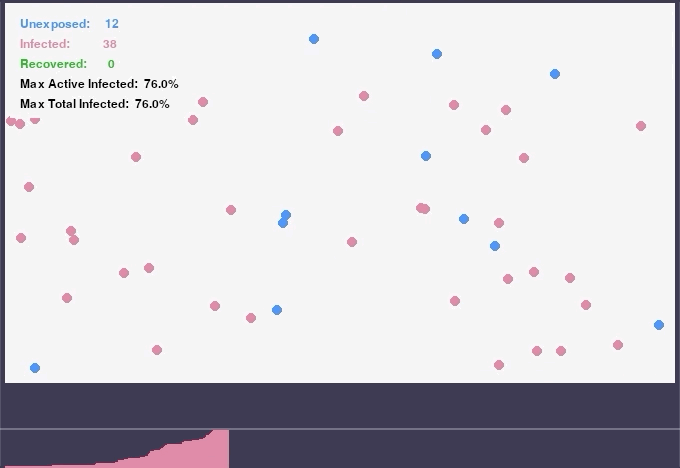
\includegraphics[width=\textwidth]{slides//New Folder/something-70}
%				\end{center}
%			\end{figure}
%		
%
%
%		\end{column}
%	\end{columns}
%
%\end{frame}








% 
 \begin{frame}{\underline{Some of my computational Projects} }
 	\begin{columns}
 		\begin{column}{0.5\linewidth}
 
 	\begin{itemize}			  \setlength\itemsep{1em}
 		
 			\item \textbf{Simulation of a Mach Zehnder interferometer as a coronagraph} : simulate image results for a telescope that use a Mach Zehnder interferometer  In collaboration with a master student in astrophysics
 		
 		\item \textbf{Higgs ML }: signal / background separation using new machinee and deep learning techniques ( RNN and Xgboost instead of BDT)
 		

 		
 		\item \textbf{....} : ( please take a look at my \faGithubSquare $ $ profile )
 		
  
 \end{itemize}
 		\end{column}
 
 		\begin{column}{0.5\linewidth}
 
 			
 			% \animategraphics[loop,width=\textwidth]{10}{slides/New Folder/something-}{0}{16}
 
 			\begin{figure}[H]
 				\begin{center}
 					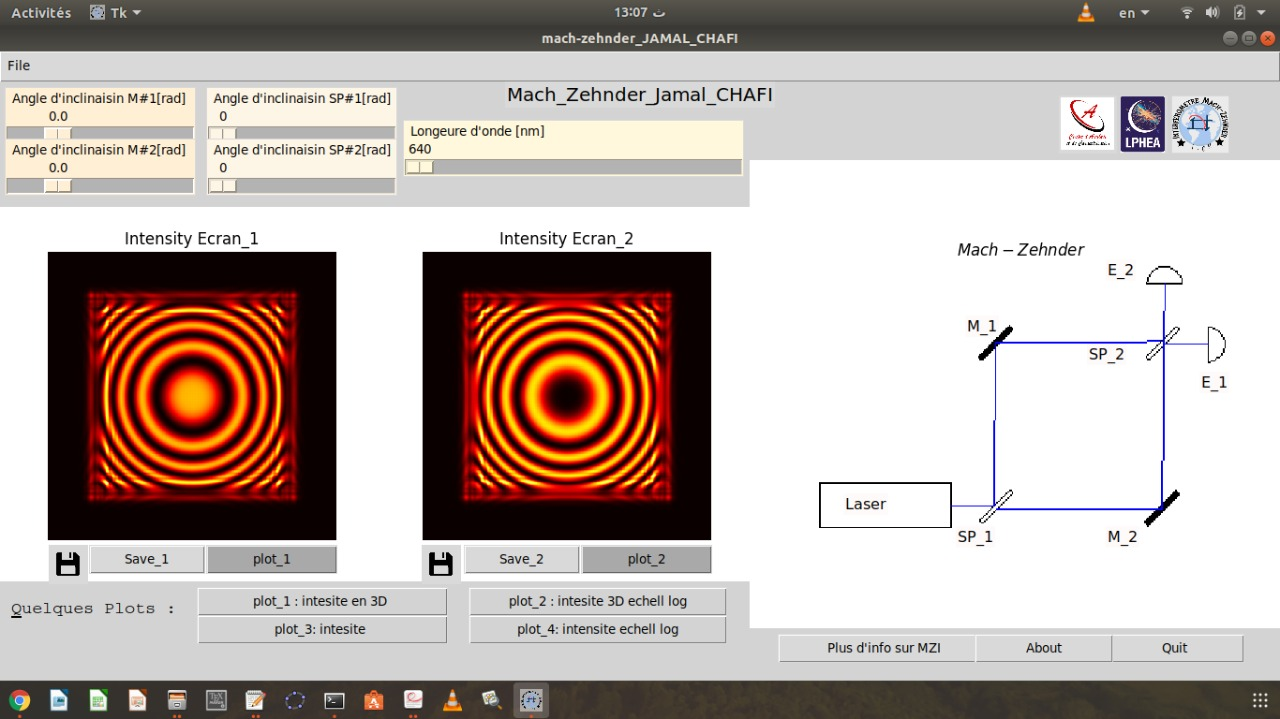
\includegraphics[width=\textwidth]{jamal}
 				\end{center}
 			\end{figure}
 		
 
 
 		\end{column}
 	\end{columns}
 
 \end{frame}
% 

{
\usebackgroundtemplate{ \centering 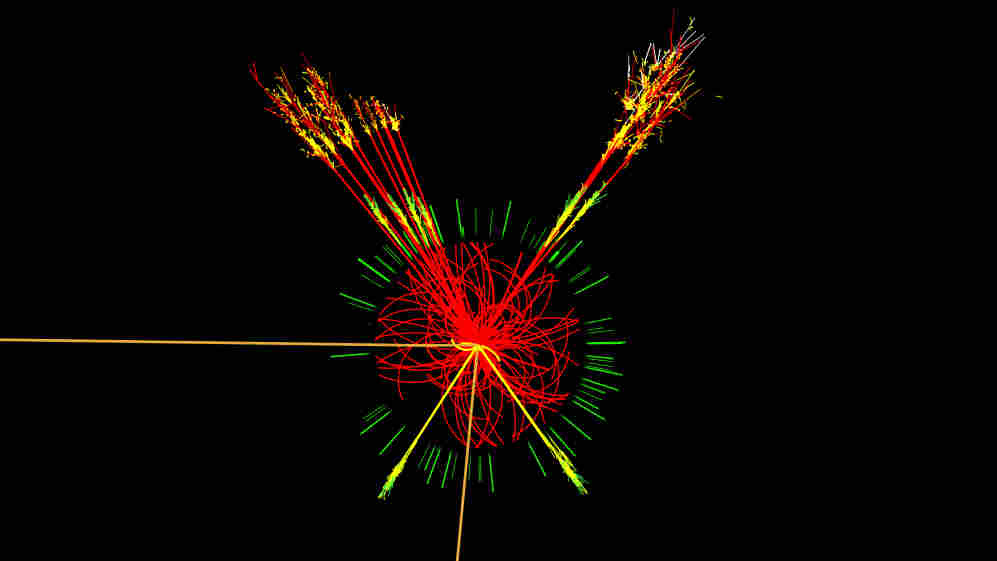
\includegraphics[height=\paperheight,width=\paperwidth]{figures/higgs}}%
\begin{frame}\frametitle{{\color{white}Finally...}}


	\centering

	{\vspace{17em} \Huge {\color{white}	\textbf{Thanks For Your Attention !!}\\}}
\end{frame}

}


%=================================================
% end presentation
%=================================================



\end{document}
